\documentclass[10pt,letter]{article}
\usepackage[utf8]{inputenc}
\usepackage{amsmath}
\usepackage{amsfonts}
\usepackage{amssymb}
\usepackage{graphicx}
\usepackage[margin=1in]{geometry}


\begin{document}

\begin{titlepage}
\title{PHYS 5794 Homework 5}
\date{March 1, 2016}
\author{Thomas Edwards}
\maketitle
\end{titlepage}

\section{Problem 1}

\subsection{Problem Statement}Write a program for fitting hypothetical Millikan’s oil-drop experimental data shown in Table 1 and
Fig.1 to a linear function, $e_n = n e_0 + \Delta e$, by using the least-squares fit or the $\chi^2$ fit, where $e_0$ and
$\Delta e$ are two parameters that need to be determined.(30 pts)
The following issues should be addressed either in the report.

(a) Construct $\chi^2$ .

(b) Construct a set of linear equations by minimization of $\chi^2$ with respect to the two unknown
parameters.

(c) Solve the set of linear equations using the Gauss elimination, LU decomposition, or singular
value decomposition method (pick one of them and specify which one was used).

(d) Write down the $e_0$  and $\Delta e$ values obtained from the fitting.

(e) Estimate the standard deviations of the fitting parameter values, and covariance of the two
parameters.

(f) Discuss how good your fit is by calculating the Q value.

(g) Print out the differences between the data and the values obtained from the model linear
function  $e_n = n e_0 + \Delta e$ after the fitting. Plot the data with the model function.

(h) If the standard deviations for the data are not provided, the value of Q would be
meaningless. By setting $\sigma_{en} =1$, compute $\chi^2$ again and check if the fitted parameter values $e_0$ and $\Delta e$ change compared to the previous case.

\subsection{Method}

This problem was solved using the $\chi^2$ fitting method discussed in class.

The fitting is done by solving the matrix equation 

$$\alpha \textbf{a} = \beta$$

for \textbf{a}, where $\alpha$ is a matrix of second partial derivatives of $\chi^2(a, b)$ with respect the two fitting parameters $a$ and $b$, $\beta$ is the vector of first partial derivative of $\chi^2(a, b)$ with respect the two fitting parameters $a$ and $b$, and $\textbf{a}$ is a vector of fitting parameters themselves. For this particular problem, the partial derivatives of the $\chi$ distribution are fairly straightforward, and follow as
\[\alpha = 
\begin{bmatrix}
S & S_x \\
S_x & S_{xx} 
\end{bmatrix},
\beta = 
\begin{bmatrix}
S_y  \\
S_{xy} 
\end{bmatrix}
\]
where

$$ S = \sum_i \frac{1}{\sigma_i^2}, \ S_x = \sum_i \frac{x_i}{\sigma_i^2}, \  S_y = \sum_i \frac{y_i}{\sigma_i^2}, \  S_{xx} = \sum_i \frac{x_i^2}{\sigma_i^2}, \  S_{xy} = \sum_i \frac{x_iy_i}{\sigma_i^2} $$.

This simplification is purely based on this fitting being a linear function, and does not hold for non-linear methods, as will be discussed in problem 2.

Further, the covariance and standard deviations for the fitting parameters are found by exploiting the relations

$$\sigma_a^2 = \frac{S_{xx}}{\Delta}, \ \sigma_b^2 = \frac{S}{\Delta},\  \text{and } cov = -\frac{S_x}{\Delta}$$

where

$$ \Delta = SS_{xx}-S_x^2 $$.

Further, the correlation coefficient is found by

$$r = \frac{cov}{\sigma_a \sigma_b} .$$

The $Q$ value is also solved for, by creating a recursive function for both $\gamma$ and $Gamma$, and then calculating

$$ Q = 1 - \frac{\gamma(\nu/2,\chi^2/2)}{\Gamma(\nu/2)}$$

where

$$ \nu = \text{Number of data points} - \text{Number of parameters} = \text{Degrees of freedom}$$

The fitting parameters $a$ and $b$ are then solved using LU decomposition, and the subsequent extra parameters are solved for after a fit has been found. The fit, along with the original data, is then plotted.

\subsection{Verification of Program}

The validity of this program was checked visually against the data given, to makes rue the fit was correct. The plot for this fit is below.

\begin{figure}[h]
  \centering
    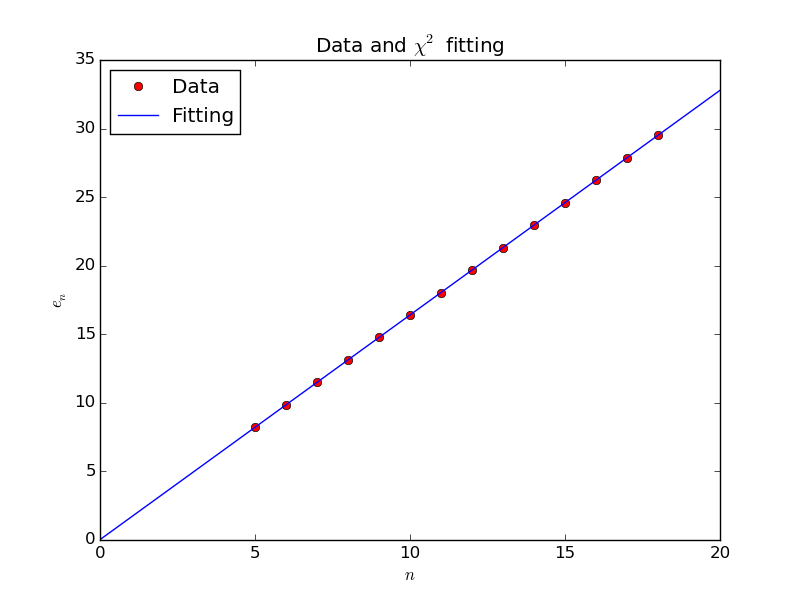
\includegraphics[width=.7\textwidth]{homework5_problem1_plot1}
  \caption{Fitting of data, where the red points are the given data and the blue is the function presented by the $\chi^2$ fitting.}
\end{figure}

As we can see from the plot, the fit appears to be very close to what is expected. Further details on the ``goodness" of the fitting are found in the data below.

\subsection{Data}

The data requested in the problem statement is below.

\begin{verbatim}
-----------------------------------------
             Chi^2 Fitting               
-----------------------------------------
*****************************************
        Values Obtained in Fitting       
*****************************************
 e_0 = 
0.0265500953703
 Delta e = 
1.63812431045
*****************************************
          Standard Deviations           
*****************************************
 sigma_a = 
0.0135542793545
 sigma_b = 
0.00114701495602
 Covariance = 
-1.47686116553e-05
 Correlation = 
-0.949935587052
*****************************************
                 Chi^2                   
*****************************************
 chi^2 = 
6.70123358753
*****************************************
                   Q                     
*****************************************
 Q = 
0.94182547217
*****************************************
   Differences between Data and Model    
*****************************************
[-0.01117165  0.02470404  0.00657973  0.00845542  0.05033111 -0.0077932
 -0.00591751 -0.00404182 -0.00216613 -0.00029044  0.00158525  0.00346094
  0.00533663  0.00721232]




-----------------------------------------
       Chi^2 Fitting (Sigma = 1)         
-----------------------------------------
*****************************************
        Values Obtained in Fitting       
*****************************************
 e_0 = 
0.0391912087912
 Delta e = 
1.6374989011
*****************************************
          Standard Deviations           
*****************************************
 sigma_a = 
0.807927752183
 sigma_b = 
0.0662993544132
 Covariance = 
-0.0505494505495
 Correlation = 
-0.943701430842
*****************************************
                 Chi^2                   
*****************************************
 chi^2 = 
0.0030903032967
*****************************************
                   Q                     
*****************************************
 Q = 
-1402988.21697
\end{verbatim}



\subsection{Analysis}

From both the printed data and the plot we see that the fitting was fairly good. The correlation itself (which would otherwise be squared) is very close to 1, and the Q value is very high. Both standard deviations are relatively low, especially considering that they are on the order of the standard deviations given for the data itself. Further, the differences shown between the data and the model are relatively small, and in some cases below $10^{-3}$.

When we remove the standard deviations from the data (by setting them equal to 1) we see that the $\chi^2$ and the Q values both become unusable. The fitting itself is similar, which is understandable considering that when $\sigma = 1$ it becomes a least-squares fitting routine that does not explain the $chi^2$ distribution.

\subsection{Interpretation}
The results of the fitting are as expected. From the problem statement, we see that the data from the Millikan oil-drop experiment does correspond to a linear function for the range of $n$ provided.

\subsection{Log}
This problem took approximatively 6 hours.

\section{Problem 2}

\subsection{Problem Statement}
Write a program to fit the following data to a nonlinear function
$y(x; a , k ) = a x e^{-k x} $by using the Levenberg-Marquardt method. You may start with an initial
guess of a = 3.1 and k = 0.4. (30 pts)

(i) Find the fitting parameters $a$ and $k$. What is your fudge factor $\lambda$? To solve the equations for
the update of the parameter values, you may consider using the Gauss elimination method or LU
decomposition method with partial pivoting or the SVD method.

(ii) Find the standard deviations
of the parameter values. 

(iii) Find the covariance of the two parameter values. 

(iv) Print out the
differences between $y_i$ and $y(x_i ; a_f , k_f )$, where $a_f$ and $k_f$ are the parameter values obtained from
the fitting. 

(v) Plot the data with the model function $y(x; a_f , k_f ) = a_f x e^{-k_f x}$, where $a_k$ and
$k_f$ are the fitting parameter values. 

(vi) Vary your initial guess of $a$ and $k$ to see if the fitted values
of $a$ and $k$ change. 

(vii) How about changing the initial value of $\lambda$ (fudge factor)? Would this affect
your final answer?

\subsection{Method}

The method for solving this problem is very similar to that of the first, with a few important modifications. In this case, the construction of $\alpha$ and $\beta$ are not as simple, since the derivatives are not simple linear relationships. Instead, we let

$$\beta_{j} = \frac{\partial\chi^2}{\partial a_{i}} = \sum_i \frac{y_i - f(x_i;\textbf{a})}{\sigma_i^2} \frac{\partial y(x_i;\textbf{a})}{\partial a_j}$$

and

$$ \alpha_{jk} = \frac{\partial^2\chi^2}{\partial a_{i} \partial a_j} = \sum_i \frac{1}{\sigma_i^2} \frac{\partial y(x_i;\textbf{a})}{\partial a_j}\frac{\partial y(x_i;\textbf{a})}{\partial a_k} $$.

It should be noted that the $\alpha$ values are a result of an approximation, where the difference between the $y_i$ and $f(x_i;\textbf{a})$ goes to 0.

An initial guess for the fitting parameters $a$ and $k$ are provided. From here, the fitting parameters are found using LU decomposition and the $\chi^2$ value is determined, as in the previous problem. Next, the diagonal of $\alpha$ is modified slightly by a ``fudge factor" $\lambda$, such that

$$\alpha_{ii} ' = \alpha_{ii}(1+\lambda) $$.

This new equation $\alpha ' \textbf{a} = \beta$ is then solved again. The solution of this modified equation is taken as $\delta \textbf{a}$. From here, $\chi^2$ is determined again for $\textbf{a}+\delta \textbf{a}$, and compared to the original $\chi^2$. If the new $\chi^2$ value is smaller than the current best solution, the new solution (including $a$ and $k$ values) is saved, and $\lambda$ is reset. Otherwise, $\lambda$ is increased to search for a good solution. This process is allowed to continue until either the change in $\chi^2$ values is small compared to some tolerance value, or if a maximum number of iterations are reached.

The covariance and standard deviation are found by taking the last good $\alpha '$ and finding the inverse. The inverse allows us to find the standard deviations by looking at the diagonal of the inverted matrix, and the covariance by taking the off-diagonal elements.

\subsection{Verification of Program}

This program was verified visually, in the plot below.

\begin{figure}[h]
  \centering
    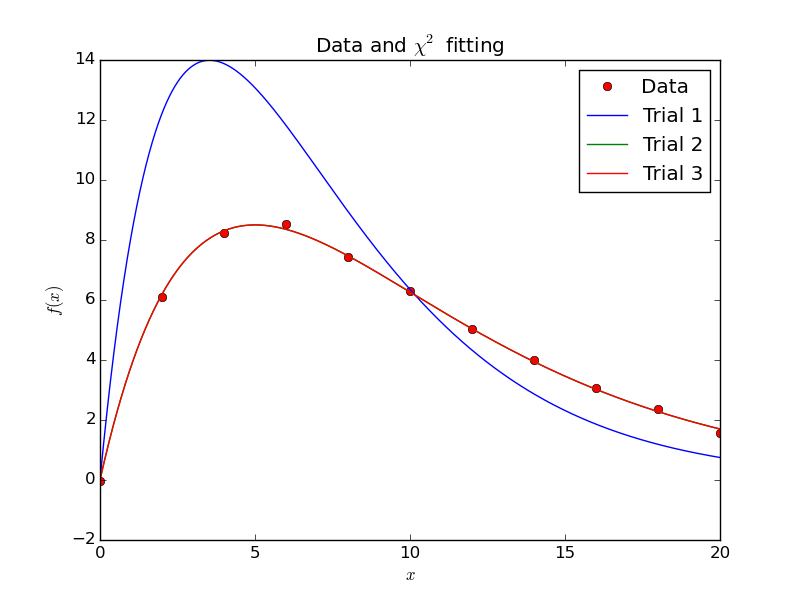
\includegraphics[width=.7\textwidth]{homework5_problem2_plot1}
  \caption{Fitting of data, where the red points are the given data and the blue, green, and red lines are the function presented by the $\chi^2$ fitting.}
\end{figure}

It is important to take a moment to explain that while the blue fit (for the original guesses) looks quite bad, it does not mean that the algorithm ran poorly. Instead, the function does fit two of the points (the first and sixth) exceptionally well.

When the guess is varied, however, the function is fit very well. More discussion on this will be given in the Interpretation portion.

\pagebreak
\subsection{Data}

The data requested in the problem statement is below.

\begin{verbatim}
-----------------------------------------
     Nonlinear Chi^2 Fitting Trial 1     
-----------------------------------------
 initial a = 
3.1
 initial k = 
0.4
*****************************************
   Standard Deviations and Covariance    
*****************************************
 std_a = 
0.00457912843076
 std_k = 
5.22287147556e-07
 covariance = 
4.30555414548e-05
*****************************************
         Fitting Parameters Found        
*****************************************
 a = 
10.7612509197
 b = 
0.282959516446
*****************************************
   Differences between Data and Model    
*****************************************
[-0.02802838 -6.11346037 -5.64548094 -3.2958361  -1.51189197 -0.0552007
  0.71617872  1.1212269   1.21625875  1.16614676  0.83208412]




-----------------------------------------
     Nonlinear Chi^2 Fitting Trial 2     
-----------------------------------------
 initial a = 
300.1
 initial k = 
0.2
*****************************************
   Standard Deviations and Covariance    
*****************************************
 std_a = 
0.00155830193101
 std_k = 
5.43749452149e-07
 covariance = 
2.69345814194e-05
*****************************************
         Fitting Parameters Found        
*****************************************
 a = 
4.61687729236
 b = 
0.199747842225
*****************************************
   Differences between Data and Model    
*****************************************
[-0.02802838 -0.08485808 -0.07240859  0.16997593 -0.03343161  0.03385268
  0.00397691  0.0446785   0.05411858  0.07404028 -0.11755578]




-----------------------------------------
     Nonlinear Chi^2 Fitting Trial 3     
-----------------------------------------
 initial a = 
300.1
 initial k = 
0.2
*****************************************
   Standard Deviations and Covariance    
*****************************************
 std_a = 
0.00155830704009
 std_k = 
5.43749302832e-07
 covariance = 
2.69346192241e-05
*****************************************
         Fitting Parameters Found        
*****************************************
 a = 
4.61688849168
 b = 
0.199748049635
*****************************************
   Differences between Data and Model    
*****************************************
[-0.02802838 -0.08487054 -0.07242185  0.16996606 -0.03343733  0.03385047
  0.00397723  0.04468039  0.05412128  0.07404326 -0.11755285]

\end{verbatim}

\subsection{Analysis}

On the surface, it appears that the fitting did not work. This is not necessarily the case, and will be discussed in the Interpretation portion.

The standard deviation are exceptionally small, which is to be expected. In particular, $k$ has a very small standard deviation, due to it's exponential dependence.

For the initial solution, the found fitting parameters are not close to the initial guesses, especially for $a$, but they are somewhat reasonable for the function we are trying to fit.  The fact that the output function (in blue) fits on the page suggests that the results is somewhat constrained. The second trial (which overlaps with the third trial) is much better, even when given a wild initial guess of $a=300.1$ and $k=0.2$. Further, the standard deviations and covariances are similar to that of the first trial.

\subsection{Interpretation}

First, it should be stated that the original guesses did not return a good fit for the data. This is not actually suggests that the algorithm was incorrect, and that instead that the derivative of the distribution for this particular case was not well suited for the initial guesses that were given.

It is apparent in the second trial, where the initial parameters are changed, that there is a much better fit that can be found. This is fine, knowing that this method can be sensitive to finding \emph{local} minimums, but not \emph{global} minimums.

Further, when $\lambda$ is varied, it is seen that the solution does not change. This is expected, but with a warning: changing $\lambda$ to make it too large may give is unruly solutions, for the same reason we were unable to find the ``correct" solution for the original guesses.
\subsection{Log}

This problem took approximately 10 hours to complete.

\end{document}